\section{Motor}\label{Maxon_Motor}
The four motors actuating the EndoWrist is sold as a bulk solution which include motor\cite{motor_motor}, gear\cite{motor_gear} and a position encoder\cite{motor_encoder}, see \figref{fig:Full_motor _dis}.
These motors are direct current (DC) motors. The main parameters for this bulk solution are listed below:

\begin{itemize}
	\item Torque constant: $10.9\frac{\text{mNm}}{\text{A}}$
	\item Nominal continues current: 0.681 A 
	\item Gearing ratio: 1:19
	\item Encoder precision: 512 counts pr. rotation. With the proper programming, see section \ref{encount}, 2048 positions can be distinguished in one rotation.
\end{itemize}

\begin{figure}[H]
	\centering
	\begin{subfigure}{.32\textwidth}
		\vspace{0pt}
		\centering
		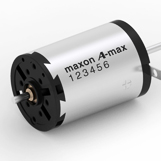
\includegraphics[width=\linewidth]{motor.jpg}
		\caption{The Maxon 110160 \newline DC motor.}
		\label{fig:motor}
	\end{subfigure}
	\begin{subfigure}{.32\textwidth}
		\centering
		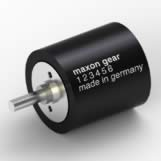
\includegraphics[width=\linewidth]{motor_gear.jpg}
		\caption{The planetary gearhead, 110356, equipped with sleeve bearing.}
		\label{fig:motor_gear}
	\end{subfigure}
	\begin{subfigure}{.32\textwidth}
		\hspace{5pt}
		\centering
		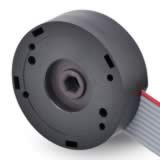
\includegraphics[width=\linewidth]{motor_sensor.jpg}
		\caption{The encoder, 201937, used for getting angular data.}
		\label{fig:motor_sensor}
	\end{subfigure}
	\caption{The combination gear disassembled}
	\label{fig:Full_motor _dis}
\end{figure}

The control of these motors are done through the ESCON controller boards, connected to the sbRIO, as shown on \figref{interface}. A detailed description is provided in \secref{sec:motor_control}.